\section{Structure}
The \textbf{Foodplan} class describes a schedule of planned meals that a user can administrate and follow.
It can consists of 0 to many meals.

The \textbf{Meal} class contains information about a meal and when to make/eat it. It consists of recipes.

\textbf{Recipes} consists of \textbf{Food}.

\begin{figure}[H]
	\centering
	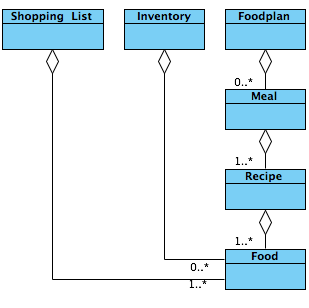
\includegraphics[width=0.50\textwidth]{Grafik/FoodPlanner/FoodPlannerClassDiagram.png}
	\caption{Relation between classes.}
\end{figure}

\fxnote{In developement..}